\chapter {Element Attributes}

%-----------------------------------------------------------------
\section{Independent and Dependent Attributes}

For convenience \bmad computes the values of some attributes based
upon the values of other attributes. For example, the \vn{volt} and
\vn{e_field} attributes of an \vn{elseparator} are calculated from
the \vn{hkick}, \vn{vkick}, \vn{l}, \vn{gap}, and \vn{beam_energy}
attributes. No attempt should be made to set or vary within a program
these dependent attributes. 
There are, however, some exceptions. For
example, the \vn{delta_e} attribute of an \vn{lcavity} is a dependent
attribute which is computed from the \vn{gradient} attribute.  If,
however, the \vn{delta_e} attribute is set in the lattice file the
\vn{gradient} will be appropriately calculated. If both \vn{delta_e}
and \vn{gradient} are set then \bmad\ generates an error message. 


Some attributes can be dependent or independent depending upon if they
appear (with non--zero values) or not in the lattice file.  For
example, If the \vn{k1} value of a \vn{quadrupole} element is set in
the lattice file then the \vn{b_gradient} attribute for that element
is a dependent variable. However, if the \vn{b_gradient} is set the
\vn{k1} attribute becomes the dependent variable. Having the
\vn{b_gradient} as the independent variable is convenient in the
situation, say, where a quadrupole's field is fixed but the beam
energy is varying. If both attributes appear then \bmad\ generates an
error message. Note the difference between a conditional dependent 
variable like \vn{b_gradient} and a dependent variable like \vn{delta_e} 
which may be set in the lattice file. Within the lattice file there
is no distinction. After a lattice has been read in and a program is
running a conditional dependent variable can be varied directly
by the program while a dependent variable cannot.

%-----------------------------------------------------------------
\section{Type, Alias and Descrip Attributes}
\label{s:string}

\vn{type}, \vn{alias}, and \vn{descrip} are labels to be attached 
to an element. \bmad\ does not directly use these labels. \vn{Type}
and \vn{Alias} can be up to 16 characters in length and \vn{Descrip}
can be up to 200 characters. The attribute strings can be enclosed in
double quotation marks ("). The attribute strings may contain
blanks. If the attribute string does not contain a blank then the
quotation marks may be omitted. In this case the first comma (,) or
the end of the line marks the end of the string. Example:
\begin{example}
  Q00W: Quad, type = "My Type", alias = Who_knows, &
                                  descrip = "Only the shadow knows"
\end{example}

%-----------------------------------------------------------------
\section{Offset, Pitch, Tilt, and Roll Attributes}
\label{s:offset}

There are up to 7 attributes that can offset a physical element
from the reference orbit. They are
\begin{example}
  x\_offset
  y\_offset
  s\_offset
  x\_pitch
  y\_pitch
  tilt
  roll
\end{example}
The exception here is the \vn{pitch} element which uses these
attributes to modify the reference orbit itself.

\vn{x_offset} translates an element in the local $x$--direction
as shown in Figure~\ref{f:pitch}. Similarly, \vn{y_offset} and 
\vn{s_offset} translate an element along the local $y$ and 
$z$--directions respectively. For a bend it is assumed that
the bend angle is small and the rotation of the local reference
axes through the bend is ignored.

The \vn{x_pitch} attribute rotates an element about the $y$--axis
so that the exit face of the element is displaced in the 
$+x$--direction as shown in figure~\ref{f:pitch}. Similarly
the \vn{y_pitch} attribute rotates an element about the $x$--axis
so that the exit face of the element is displaced in the 
$+y$--direction. The rotations
are about the center of the element which is in contrast to the 
\vn{dtheta} and \vn{dphi} misalignments of \mad\ which rotate
around the entrance point. In terms of rotation angle
\begin{example}
  x_pitch =  dtheta
  y_pitch = -dphi
\end{example}
In both \bmad\ and \mad\ offsets are applied before pitches.
\begin{figure}
  \centering
  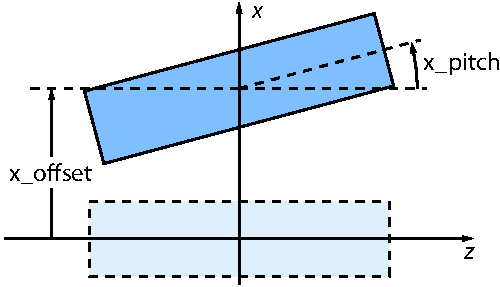
\includegraphics{pitch.psfig}
  \caption{Geometry of Pitch and Offset attributes}
  \label{f:pitch}
\end{figure}

\begin{figure}
  \centering
  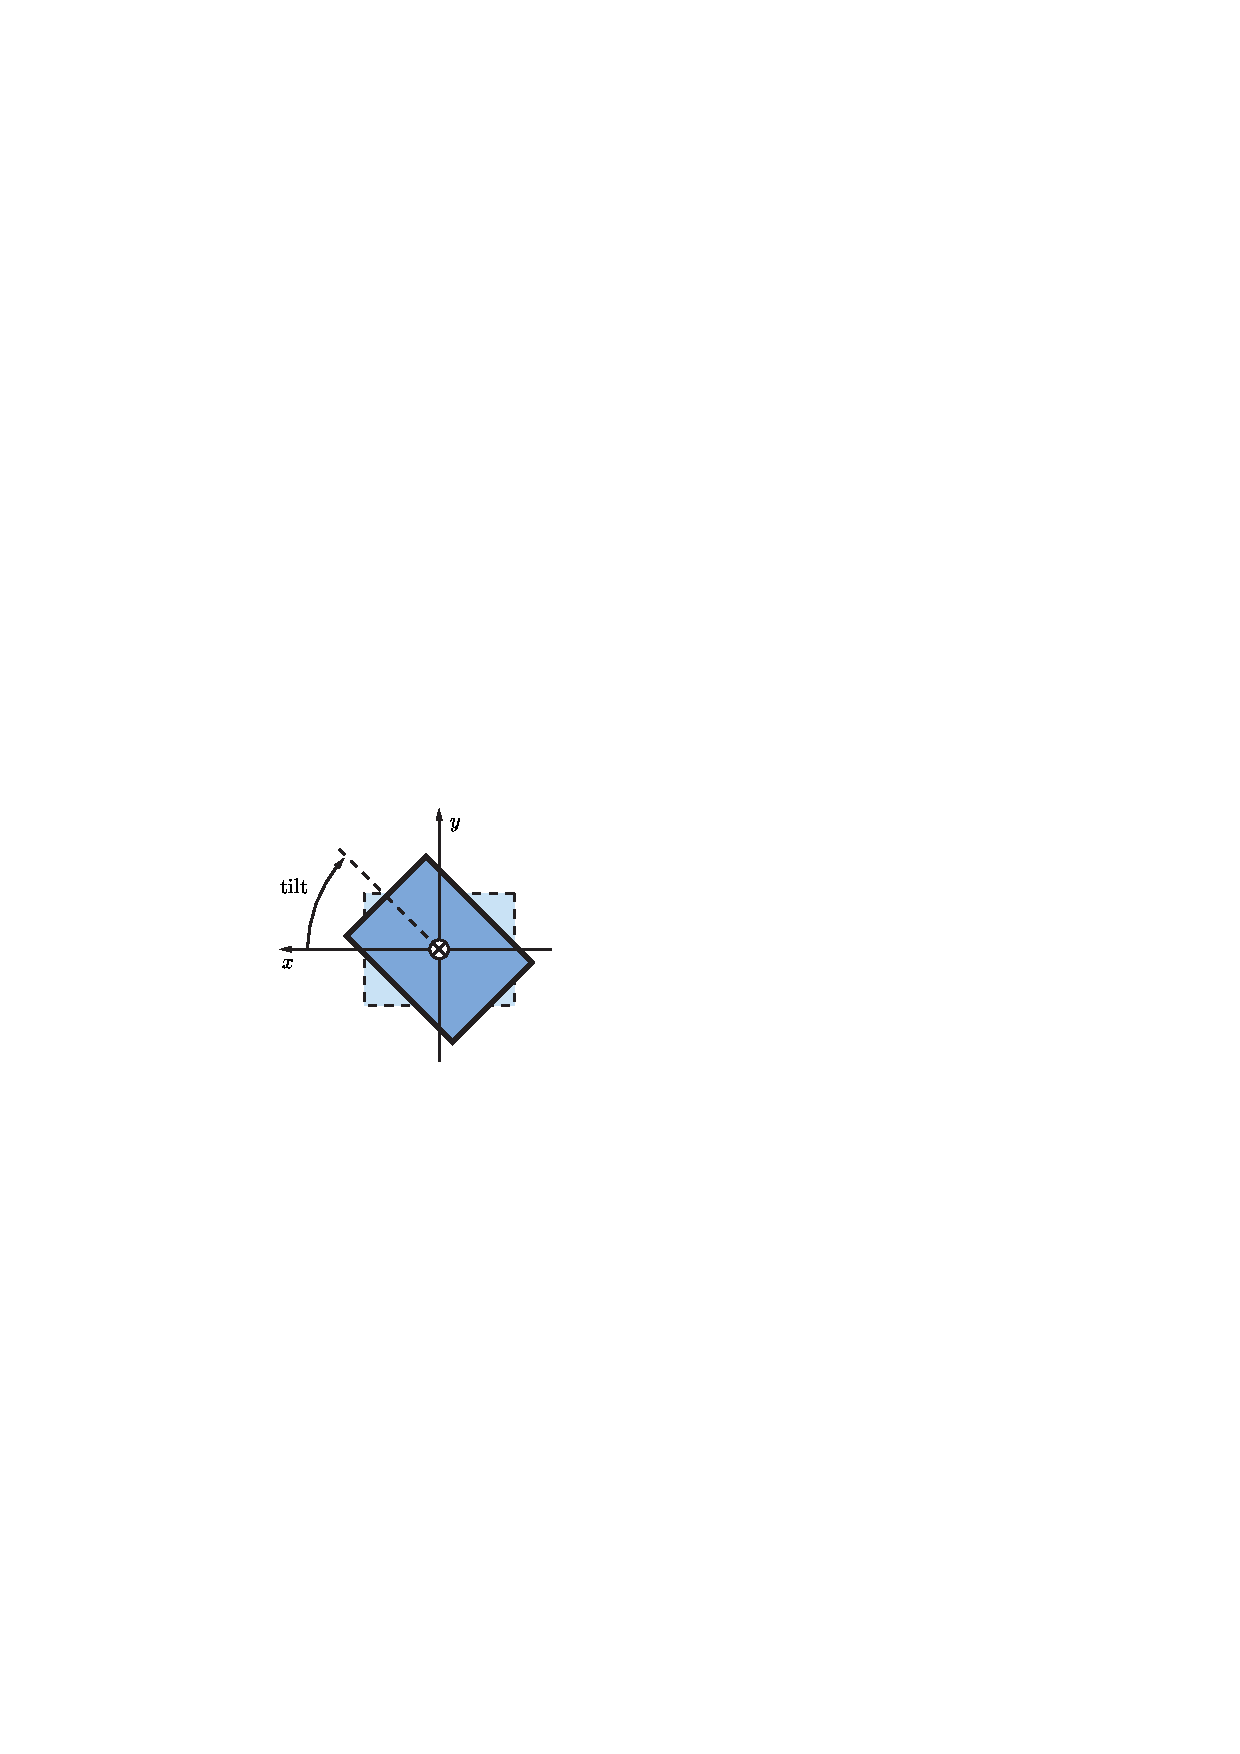
\includegraphics{tilt.psfig}
  \caption{Geometry of a Tilt}
  \label{f:tilt}
\end{figure}

The tilt attribute rotates the element in the $(x, y)$ plane as
shown in figure~\ref{f:tilt}. For a bend the rotation axis is the
$z$-axis at the entrance face. The reference orbit is also rotated
with the element. A bend with a tilt of $pi/2$ will bend a beam
upward vertically. The \vn{hkick} and \vn{vkick} attributes are
not affected by \vn{tilt} except for \vn{Kicker} and \vn{ElSeparator}
elements
Like MAD, \bmad\ allows the use of the \vn{tilt} attribute without
a value to designate a skew element. For example
\begin{example}
  q1: quad, l = 0.6, x_offset = 0.03, y_pitch = 0.001, tilt
\end{example}
Default tilts can be used for \vn{rbend}, \vn{sbend}, \vn{sol_quad},
\vn{quadrupole}, vn{sextupole}, and \vn{octupole} elements.
The default tilt is $\pi/n$ where $n$ is the number of poles of the
element (bends have 2, quadrupoles have 4, etc.) 


The \vn{roll} attribute is only used for bends
and rotates the bend, along an axis that runs through the entrance
point and exit point as shown in figure~\ref{f:roll}. A \vn{roll} 
does not affect the reference orbit. The major effect of a \vn{roll}
is to give a vertical kick to the beam.
\begin{figure}
  \centering
  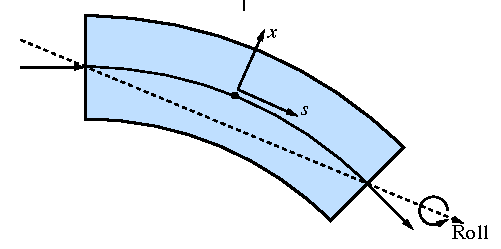
\includegraphics{roll.psfig}
  \caption{Geometry of a Roll}
  \label{f:roll}
\end{figure}


%-----------------------------------------------------------------
\section{Hkick, Vkick, and Kick Attributes}
\label{s:kick}

\vn{kick}, \vn{hkick}, and \vn{vkick} attributes are the integrated
kick of an element in radians. \vn{kick} is only used for \vn{Hkicker}
and \vn{Vkicker} elements. All other elements that can kick use 
\vn{hkick} and \vn{vkick}. The \vn{tilt} attribute will only rotate
a kick for \vn{Hkicker}, \vn{Vkicker}, \vn{ElSeparator} and \vn{Kicker}
elements. This rule was implemented so that, for example, the 
\vn{hkick} attribute for a skew quadrupole
would represent a horizontal steering.

%-----------------------------------------------------------------
\section{Aperture and Limit Attributes}
\label{s:limit}

\begin{figure}
  \centering
  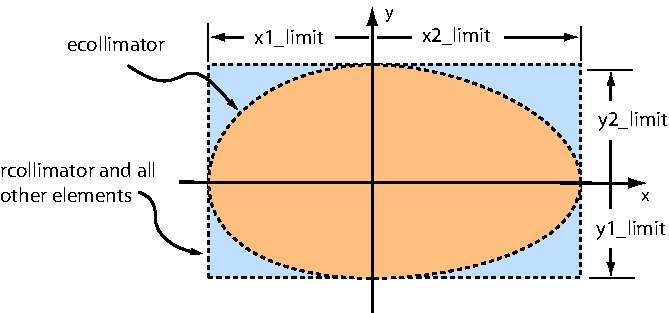
\includegraphics{apertures.psfig}
  \caption{Apertures for ecollimator and rcollimator elements}
  \label{f:limit}
\end{figure}

\vn{x_limit}, \vn{y_limit} specify the half--width of the 
aperture of an element as shown in figure~\ref{f:limit}. 
The aperture is evaluated at the exit
face only of the element. A zero \vn{x_limit} or \vn{y_limit}
is interpreted as no aperture in the $x$ or $y$ direction.
offsets move the aperture but not pitches or tilts.

\vn{aperture} attribute supersedes
any \vn{x_limit} and \vn{y_limit} values and sets \vn{x_limit} and
\vn{y_limit} equal to the value of \vn{aperture}.

\noindent
Example:
\begin{example}
  q1: quad, l = 0.6
  q1[x_limit] = 0.03
  q1[y_limit] = 0.03
  q1[aperture] = 0.03  ! equivalent to the proceeding 2 lines.  
\end{example}

%-----------------------------------------------------------------
\section{Transfer Maps via Integration}
\label{s:integ}

One way to create a transfer map through an element is to divide the
element up into slices and then to propagate the transfer
map slice by slice.
There are several ways to do this integration. The Boris and Runge--Kutta 
methods integrate the equations of motion to give the zeroth order
transfer map which is just the particle orbit.
Symplectic integration using Lie algebraic techniques, on the other hand, 
can generate maps to any order.
The \vn{num_steps} attribute determines the number of slices. This is
applicable to \vn{Boris}, \vn{Symp_Lie_Bmad}, and \vn{Symp_Lie_PTC}
integration. 

\vn{integration_ord} is the order of the integration formula for 
\vn{Symp_Lie_PTC}. Possible values are
\begin{example}
  integration\_ord = 2 (default), 4, or 6
\end{example}
Essentially, an integration order of $n$ means that the error in an 
integration step scales as $dz^{n+1}$ where $dz$ is the slice thickness.
For a given number of steps a higher order will give more accurate results
but a higher order integrator will take more time per step. It turns out
that for wigglers, after adjusting \vn{num_steps} for a given accuracy, 
the order 2 integrator is the fastest. This is not surprising given the
highly nonlinear nature of a wiggler. Note that \vn{Symp_Lie_Bmad} always
uses a order 2 integrator.

\vn{Adaptive_Boris} and \vn{Runge_Kutta} use adaptive step
control independent of \vn{num_steps}. These methods use the \vn{rel_tol} and
\vn{abs_tol} attributes to try to keep the estimated error of the integration
such that
\begin{example}
  error < abs\_tol + |orbit| * rel_tol
\end{example}
lowering the error bounds makes for greater accuracy (as long as round-off 
doesn't hurt) but for slower tracking. 

\vn{Boris}, \vn{Adaptive_Boris}, and \vn{Runge_Kutta} tracking all use
as input the electric and magnetic fields of an element. The


%-----------------------------------------------------------------
\section{Length Attributes}
\label{s:l}

\vn{l} is, for all elements except \vn{RBend}s, the path length 
of the reference particle.
Note that for wigglers this is not the same as the path length for
a particle with the reference energy starting on the reference orbit.

%-----------------------------------------------------------------
\section{Symplectify Attribute}
\label{s:symp}

A linear transport matrix may be non--symplectic for a number of reasons.
For example, the linear matrix that comes from expanding a Taylor Map
around any point that is not the origin of the map is generally not 
symplectic. The transfer matrix for an element can be symplectified by
setting the \vn{symplectify} attribute to True. See section \ref{s:symp_method}
for details on how a matrix is symplectified.


%-----------------------------------------------------------------
\section{Is\_on Attribute}
\label{s:is_on}

The \vn{is_on} attribute is used to turn an element off. Turning
an element off essentially converts it into a drift. This is not
generally used in a lattice file but a program can use the attribute
for, say, calculating the Twiss parameters which needs to be done
with the RF cavities off. Example
\begin{example}
  q1: quad, l = 0.6, k1 = 0.95
  q1[is_on] = False
\end{example}
Note: \vn{is_on} does not affect any apertures that are set.